\chapter{TeXstudioの設定}

TeXstudioを使用する前に、「オプション」メニュー(Mac OS Xでは「好みの設定」)
の「TeXstudioの設定」を通じてエディターとLaTeX関連のコマンドの設定をすべきである。
注意すべきは詳細には2段階あることだ。
より高度なオプションやあまり使用しないオプションは、
左下隅の「高度なオプションの表示」にチェックをした場合にのみ表示される。

\section{エディターの設定}

エンコーディングとしてUTF8を使用したくない場合には、
新規ファイルに対する既定のエンコーディングを変えることができる
(「TeXstudioの設定」-\textgreater{} 「エディタ」 -\textgreater{} 「既定のフォントエンコーディング」)。
忘れずに文書中のプリアンブルで同じエンコーディングをセットするように
(例:UTF8を使用している場合、\verb+\usepackage[utf8]{inputenc}+)。

TeXstudioはUTF8とlatin1エンコーディングファイルを自動検出できるが、
既存の文書で異なるエンコーディングを使用する場合は開く前に設定ダイアログでエンコーディングを指定する必要がある(そして自動検出も無効にする必要がある)。

\begin{itemize}
\item
  「折りたたむ」はエディターのコード折りたたみ機能を有効/無効化する(テキストのセクションを隠す)。
\item
  選択ボックス「字下げモード」では、
  Enterキーを入力後同じインデントの行にインデントされる行を揃えるか、
  TeXstudioの自動インデントに任せるかを選択できる。
\end{itemize}

\begin{figure}[H]
  \centering
  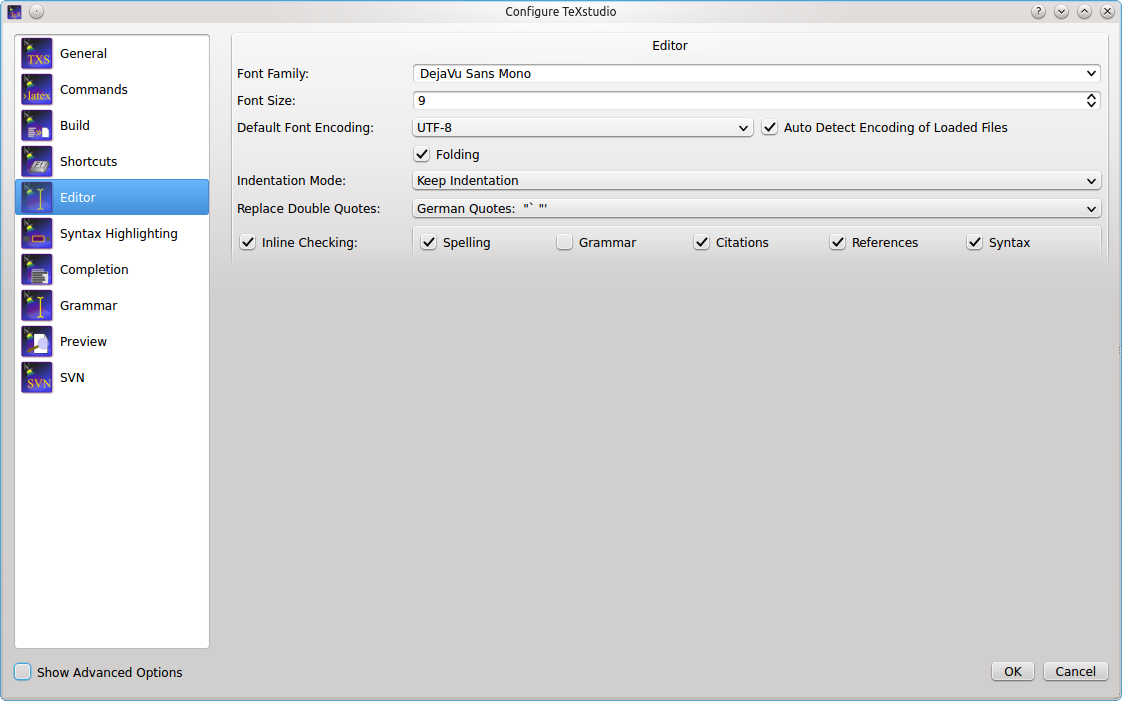
\includegraphics[width=.8\linewidth]{configure_editor.png}
  \caption{エディターの設定}
\end{figure}

\section{LaTeX関連コマンドの設定}

LaTeX関連コマンドのパスが間違っているとTeXstudioでの文書のコンパイルができない。

既定の設定は最近の標準的なLaTeXディストリビューションで機能するが、
それらを変更しても良い(「TeXstudioの設定」 -\textgreater{} 「コマンド」)。
コマンドを変更するには、
単に対応する行の終わりのボタンをクリックしてファイルブラウザでコマンドを選択すれば良い:
TeXstudioはコマンドの構文に自動的に適応する。

\textbf{\%}文字は拡張子なしのファイル名を表し、
\textbf{@}文字は現在の行番号に置換される。
更にオプションが必要なら(例:絶対パス)、
設定ダイアログの下部の説明を見て\textbf{?}を使用する。

%\hyperref[\ref{}]{順方向/逆方向検索}
\nameref{sec:search}の節では一般的なビューワーのコマンド例がいくつか挙げられている。
また、右側の「規定値に戻す」ボタンで初期設定にいつでも戻すことができる。

\begin{figure}[H]
  \centering
  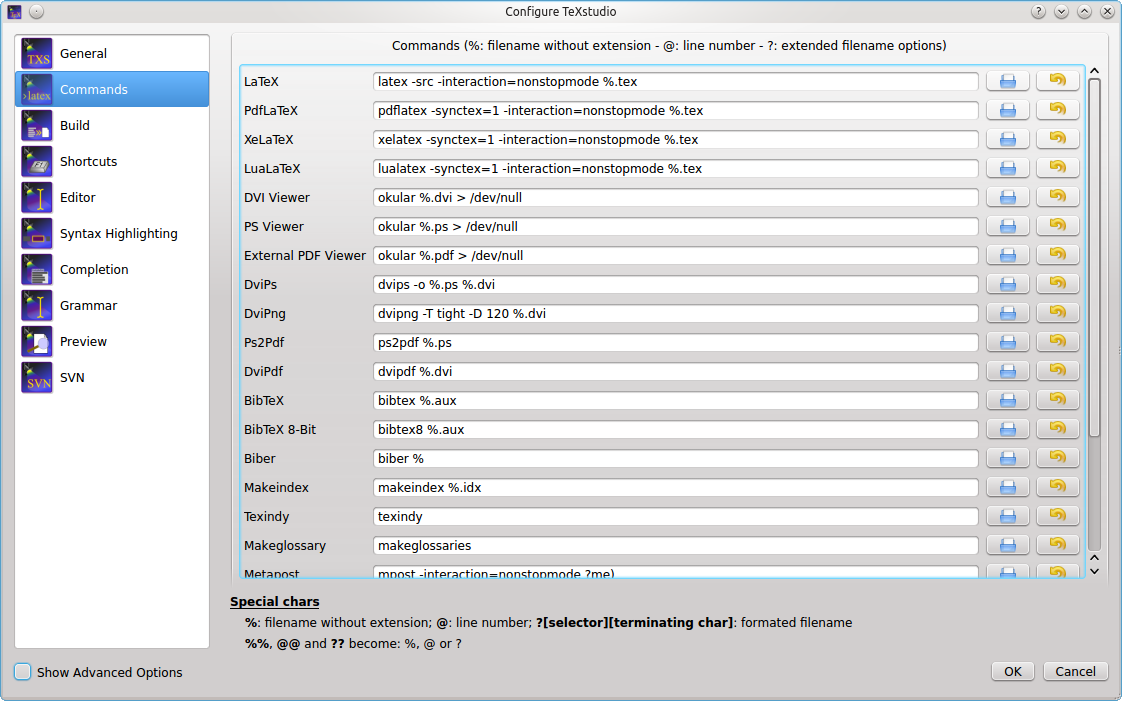
\includegraphics[width=.8\linewidth]{configure_commands.png}
  \caption{コマンドの設定}
\end{figure}

\section{ビルドシステムの設定}

TeXstudioではLaTeXを変換する一般的なコマンドが提供されている。

既定の設定では``pdflatex''と組み込みのPDFビューワーを使用する。
また、別の参考文献変換器と同様に他のコマンドやビューワーを選択することができる。

「組み込みPDFビューワー」ではPDF文書を閲覧する際に新しくウィンドウは開かれず、
エディターのテキストの隣に直接表示される。

有益な別の方法として``latexmk''をコンパイルコマンドとして使用する方法がある(システムにコマンドがインストールされている場合)。
``latexmk''ではbiblatexと索引で依存関係を非常にうまく扱える。

更に、高度なオプションでは一般的には必要ないより詳細なカスタマイズを行える。

\begin{figure}[H]
  \centering
  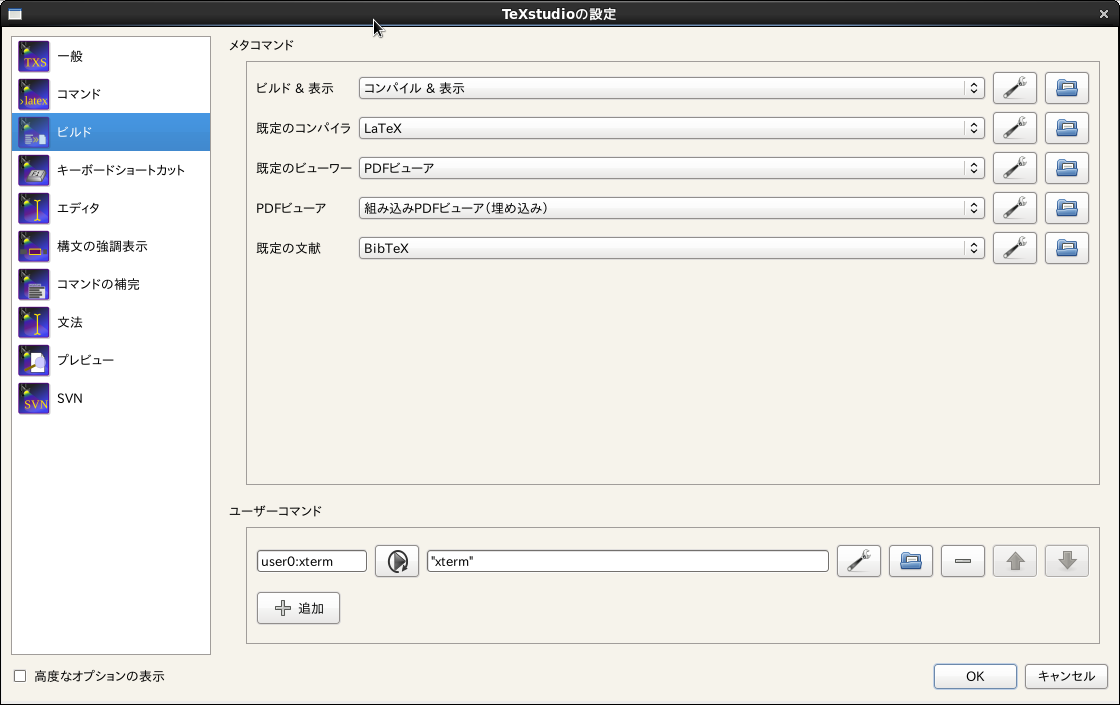
\includegraphics[width=.8\linewidth]{configure_build.png}
  \caption{ビルドシステムの設定}
\end{figure}

ここでユーザーコマンドを「追加」することで定義できる。
各々のユーザーコマンドには``user\%n:''のような名前がつく(``\%n''は数字)。
コロンの後にはツールメニューで表示される名前を記述できる。
ユーザーコマンドはショートカット(alt+shift+F\%n)または
ツールメニュー(ツール/ユーザー)のいずれかで実行できる。

ユーザーコマンドは既知のコマンドを利用可能なコマンドのリストから選択して組み合わせてもよい。
この場合スパナマークをクリックすると選択可能になる。

別な方法としては、ファイルシステムを通じて直接コマンドを選択してもよい。

\begin{figure}[H]
  \centering
  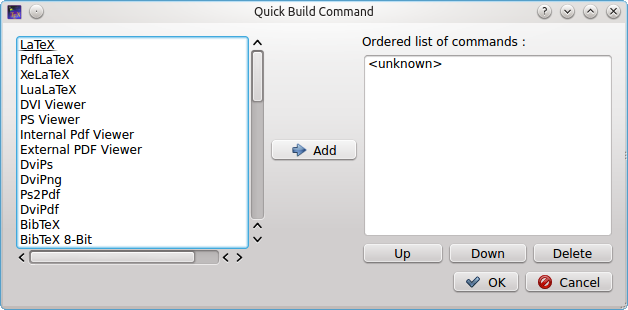
\includegraphics[width=.8\linewidth]{doc21.png}
  \caption{既知のコマンドからのユーザーコマンドの設定}
\end{figure}

\subsection{ビルドシステムの高度な設定}

高度なオプションを表示するようにしている場合、
ビルドシステムをより詳細に設定することができる。

すべてのtxs(TeXstudio)コマンドは呼び出すべき外部プログラム/LaTeXコマンドと
他のtxsコマンドのリストとなっている。
外部プログラムは通常のコマンドラインで呼び出すことができるが、
ID``foobar''を持つtxsコマンドは\texttt{txs:///foobar}で呼び出す。

リストのコマンドは単なる区切りである``\textbar{}''で区切られる
(``\textbar{}''はあるプログラムからの標準出力を
次のプログラムの標準入力へ渡す「パイプ」\emph{ではない})。

これらtxsコマンドにはそれぞれ一意的なIDが付けられ、
「通常の」コマンドの、あるいは編集ボックスではユーザーコマンドの名前のツールチップとして表示される。
いくつかの重要なコマンドは
よく使用される: \texttt{txs:///quick}(ビルド&表示、以前のクイックビルド)、
 \texttt{txs:///compile}(既定のコンパイラ)、
 \texttt{txs:///view} (既定のビューワー)、 \texttt{txs:///latex}(LaTeX)、
 \texttt{txs:///pdflatex} (pdfLaTeX)、 \texttt{txs:///view-pdf}(既定のPDFビューワー)、
 \texttt{txs:///view-pdf-external} (外部PDFビューワー)。

例えば、典型的なビルド設定ではF1を押して\texttt{txs:///quick}を呼び出すと、
\texttt{txs:///compile}が呼ばれ
(まず実際にpdfLaTeXを実行する\texttt{txs:///pdflatex}が呼ばれる)、
そして\texttt{txs:///view}が呼ばれて(\texttt{txs:///view-pdf}が呼ばれ、
それによって\texttt{txs:///view-pdf-internal}が呼ばれる)、PDFが表示される。

コマンド設定ページでコマンドとして定義されたコマンドと、
ビルド設定ページでビルドとして定義されたコマンド、
ユーザーコマンドとして定義されたコマンドには違いはない。
インターフェースの単純化のためにGUI側で区別しているだけである。

これは、前の定義を無視してあらゆるコマンドを望むように変更できる
(iniファイルを編集してIDを変えることさえできる)という事でもある。

しかし、常に定義されている三つの内部コマンドがあり、
それらは呼び出すことのみ可能で変更はできない:

\begin{table}[H]
  \centering
  \caption{TeXstudioで定義済みの内部コマンド}
  \begin{tabularx}{\linewidth}{lX}
    \hline
    \texttt{txs:///internal-pdf-viewer} & 現在の文書に対して内部ビューワーを開く\\
    \texttt{txs:///view-log} & 現在の文書に対してログファイルを閲覧する\\
    \texttt{txs:///conditionally-recompile-bibliography}
      & bibファイルが変更されているか確認して、
      変更されている場合\texttt{txs:///recompile-bibliography}を呼ぶ\\
    \hline
  \end{tabularx}
\end{table}

内部PDFビューワー(\texttt{txs:///internal-pdf-viewer})には
動作を変更するために次のオプションを使用することもできる:

\begin{table}[H]
  \centering
  \caption{内部PDFビューワーのオプション}
  \begin{tabularx}{\linewidth}{lX}
    \hline
    \texttt{--embedded} & ビューワーを埋め込みで開く\\
    \texttt{--windowed} & ビューワーを別枠で開く
      (オプションが与えられてない場合の規定値)\\
    \texttt{--close-(all\textbar{}windowed\textbar{}embedded)}
      & すべての開いているビューワーを閉じるか、
      あるいは特定のビューワーだけを閉じる\\
    \texttt{--preserve-existing} & 既存のビューワーを変更しない(つまり、
      常に新しいビューワーを開く)\\
    \texttt{--preserve-(embedded\textbar{}windowed)}
      & 既存の埋め込み/別枠ビューワーを変更しない\\
    \texttt{--preserve-duplicates} & 最初に開いたビューワーでのみPDFを開く\\
    \texttt{--(no-)auto-close} & 対応するtexファイルを閉じた時に
      ビューワーも閉じるかどうか(既定:埋め込みの場合自動的に閉じる)\\
    \texttt{--(no-)focus} & ビューワーを開いた時に
      ビューワーに焦点を移すかどうか(既定:別枠の場合焦点を移す)\\
    \hline
  \end{tabularx}
\end{table}

また、呼び出されるサブコマンドの引数を引数変更子または新しい引数の追加で変更することもできる。
これらの変更子は呼び出しリストを通じて渡されるので、
直接呼び出されるサブコマンドが別のコマンドの単なるラッパーでも、
最終的に呼び出されるプログラムの引数は常に変更される:

\begin{table}[H]
  \centering
  \caption{コマンドのオプションの例}
  \begin{tabularx}{\linewidth}{lX}
    \hline
    \texttt{txs:///foobar --xyz} & \texttt{xyz}オプションを追加\\
    \texttt{txs:///foobar{[}--xyz=123{]}}
      & \texttt{xyz}オプションの値を123に変更(つまり、
      \texttt{foobar}で定義されたあらゆる\texttt{xyz}オプションを削除して変更)\\
    \texttt{txs:///foobar\{--xyz=123\}}
      & 他の値を持つ\texttt{xyz}オプションを無視して、
      \texttt{foobar}コマンドラインから\texttt{--xyz=123}を削除\\
    \texttt{txs:///foobar\{--xyz\}} & 値にかかわらず、
      あらゆる\texttt{--xyz}オプションを\texttt{foobar}コマンドラインから削除\\
    \texttt{txs:///foobar\{\}} & 実行可能ファイル名のみ残して、
      すべてのオプションを\texttt{foobar}コマンドラインから削除\\
    \hline
  \end{tabularx}
\end{table}

最後に、iniファイルを変更することでしか変えられない隠しオプションもある:
Tools/Kind/LaTeX、 Tools/Kind/Rerunnable、 Tools/Kind/Pdf、
Tools/Kind/Stdout、 Tools/Kind/Viewer。
これらはそれぞれLaTeXコンパイラ(例えば、後にログを表示する)、
再実行可能(警告がある場合にコマンドを繰り返し呼び出す)、
PDF生成器(例えば、pdflatex)、標準出力へ出力するコマンド(例えば、bibtex)、
そしてビューワー(例えば一度だけ開く)として扱われるコマンドのリストである。

\section{一般的な事項の設定}

このパネルではいくつかの一般的な外見の設定を行うことができる。

\begin{itemize}
\item
  TeXstudioでは「スタイル」と「配色」を選択できる。
  「配色」のモダンはtexmaker 1.9に似ている。
\item
  記号リストは「タブ形式」で表示されるか(以前の形式、タブ形式が有効な場合)、
  あるいは記号の空きを多くするため記号リストのそばの小さな記号タブとして表示される。
\item
  ログビューワーもエラー一覧表やログビュー、
  プレビューワーなどの間をより速く移動できるようにタブ形式で表示される。
\item
  メニューの言語をシステムの設定を無視して直接変更することができる。
\end{itemize}

\begin{figure}[H]
  \centering
  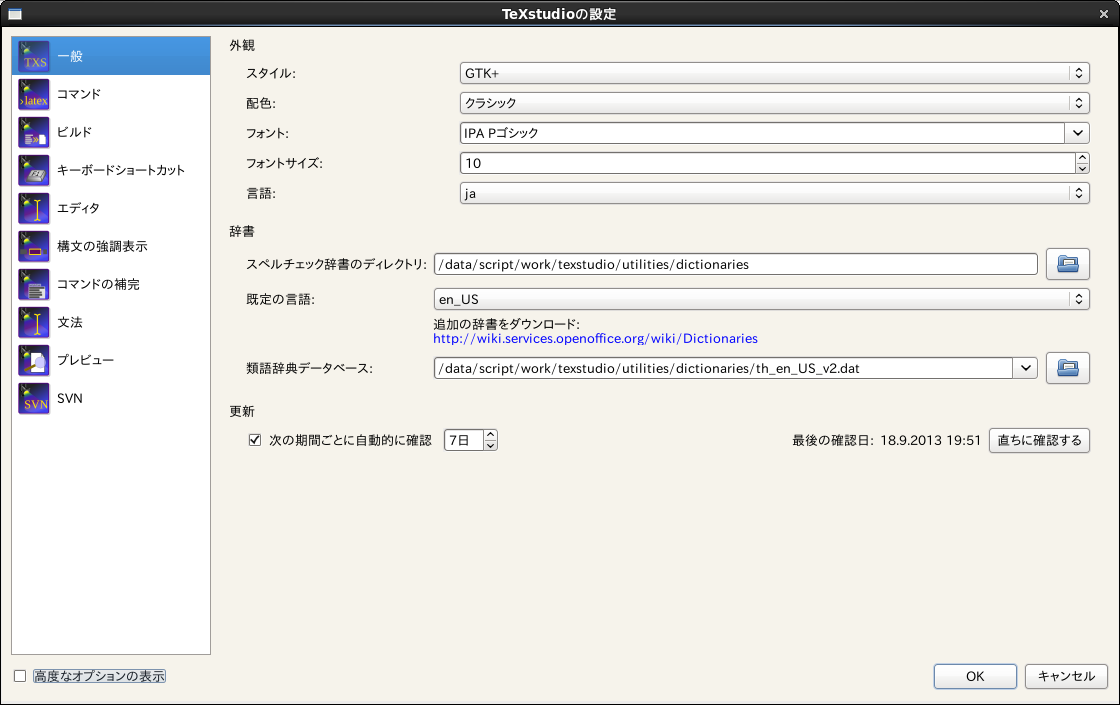
\includegraphics[width=.8\linewidth]{configure_general.png}
  \caption{一般的な設定}
\end{figure}

\subsection{スペルチェッカーの設定}

TeXstudioでは文字入力中にスペルチェックが行われる。
入力されたテキストがLaTeXコマンドの場合、
そのテキストがチェックされるべき自然言語なのか、
そのままにしておく単なるコマンドオプションなのかを
決めるためにTeXstudioではコマンド補完リストから情報が渡される。
既知のLaTeXコマンドだけがオプションでチェックされる!
既知のコマンドやパッケージについてのさらなる情報については、
%\hyperref[SECTION040]{補完}
\nameref{sec:completion}の節を参照せよ。

スペルチェッカーではOpenOffice.orgの辞書が用いられる。
初期状態ではGPLフランス語、イギリス英語、
ドイツ語の辞書がTeXstudioに同梱されている。
他の辞書は\href{http://wiki.services.openoffice.org/wiki/Dictionaries}{http://wiki.services.openoffice.org/wiki/Dictionaries}からダウンロードできる。
すべての辞書はひとつのディレクトリに保存される。

簡便のために、TeXstudioではスペルチェッカーの言語を好きに選択できる。
しかし、別の言語で書かれたファイルに対して頻繁に作業する場合規定の振る舞いを上書きしたいと思うかもしれない。
これを行うには二つの方法がある。
一つ目はステータス行の言語メニューを通じてファイルの言語を明示する方法だ。
この設定はファイルを閉じると即座に失われる。
ファイルの言語を永続的に保存するために、
TeXstudioは特別な「マジックコメント」
\textbf{\texttt{\% !TeX spellcheck = de\_DE}}をサポートしている。
このコメントがファイルにある場合、ファイルを開くとその言語に自動的に設定される。

\begin{figure}[H]
  \centering
  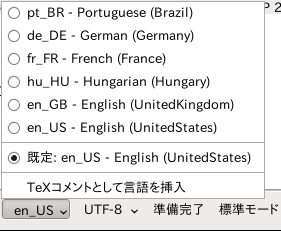
\includegraphics{spellcheck_menu.png}
  \caption{スペルチェックメニュー}
\end{figure}

注記:Ctrl+Shift+F7でのスペルチェックはカーソル位置から開始されるのであって、
文書の最初からではない。
\\

もし対話式のスペルチェッカーが有効な場合(既定)、
間違って綴られた単語すべてに赤い波下線が引かれる。
その単語で右クリックすると、考えられる訂正語のリストのメニューが表示される。
このコンテキストメニューでは無視するリストにその単語を追加することもできる。
使用している辞書がとても大きい(${}>5\mathrm{MB}$)場合、
コンテキストメニューを開いて考えられる候補を表示するのに数秒かかるかもしれない。
もし候補が不必要なら、右クリック中にShiftを押すと待つ必要がなくなる。
\\

辞書の内部構造が複雑である(例えば、
様々な変化形を持つ単語を生成する規則を含む)ので、
単純に単語を辞書に追加することはできない。
そのかわり辞書に単語がない場合、
その単語を無視するリストに追加してスペルチェッカーが何も言わないようにすることができる。
無視するリストは通常辞書と同じディレクトリに保存される。
それは拡張子が``.ign''のプレーンテキストファイルである。
もし辞書と同じディレクトリに保存できない(例えばアクセス権限がない)場合、
そのリストはユーザーの設定ディレクトリに保存される。

\subsection{類語辞典の設定}

類語辞典ではOpenOffice.org 2.xのデータベースを使用している。
GPLのフランス語、アメリカ英語、
ドイツ語のデータベースのみがTeXstudioに同梱されている。

ユーザーは次の場所から他のデータベースをダウンロードできる:
\href{http://wiki.services.openoffice.org/wiki/Dictionaries}{http://wiki.services.openoffice.org/wiki/Dictionaries}

\subsection{LaTeX構文チェッカーの設定}

LaTeX構文チェッカーでは、
コマンドが正しいかどうか判断するために考えられる完全なコマンドのリストを利用している。
更に、そのコマンドリストには、コマンドがその文脈で有効かどうか、
数式モードでのみ有効かあるいは表モードでのみ有効かを決めるための追加情報が部分的に含まれている。

\subsection{文法チェッカーの設定}

文法チェッカーは\href{http://www.languagetool.org/}{LanguageTool}の
標準的なhttp APIに基づいていて、LanguageTool(LT)とJavaを別個にインストールする必要がある。

一度LanguageToolをインストールすると、
LanguageToolのスタンドアローンアプリケーションを起動し、
その後TeXstudioを起動することで文法チェッカーを利用できる。
LanguageToolはアドレスがhttp://localhost:8081/である
ローカルで起動するサーバーを作成し、TeXstudioは起動時にそこに自動的に接続される。
接続が確立されたら、すべての入力された段落がLTに送られ、
ちょっとした後に考えられる文法上の間違いが強調表示される。

TeXstudioでLanguageToolを自動的に起動させるには、
設定ダイアログの文法ページでLT jarのパスを入力する必要がある。
Javaの実行ファイルが既定のPATHにない場合、そのパスもそこで設定する必要がある。

高度な設定モードでは、あるLTの規則を「特別」として特徴づけすることもできる。
その「特別」な規則に一致したものは異なる/カスタマイズ可能な方法で強調表示される。
これは、例えばLTですべての動詞またはすべての副詞を強調表示する
独自の規則を作成することで、文体の解析を行うのに有益である。

LanguageToolとは独立して、
TeXstudioでは繰り返しの悪い(不正確な/俗語的な)単語もチェックされる。
繰り返しの確認では、後ろのいくつかの単語を見て、
身近なところの短い単語の繰り返しや前方10単語までの長い単語の繰り返しが
しるし付けされる。
これらの距離や長さは高度な文法設定のページで変更できる。

\section{自動補完の設定}\label{sec:completion}

TeXstudioでは、補完用の既知のコマンドの数をかなり増やした、
kileの補完単語のリストを採用している。
構文チェックだけでなく補完の有効なコマンドリストを選択するため、
TeXstudioでは\verb+\documentclass+と\verb+\usepackage+が使われていることが認
識される。
しかし、TeXstudioでは
「TeXstudioの設定」 -\textgreater{} 「コマンドの補完」で追加の単語リストを選択することができる。
単語リストの名前とパッケージ名は対応関係がある。
例えばリストlatex.cwlは標準的なLaTeXコマンドを含んでいる。

自動補完に関連して、TeXstudioでは挙動を好みに合わせることができる。
オプションは次のものが利用できる:

\begin{itemize}
\item
  補完の有効化:これは自明である
\item
  大文字と小文字の区別:例えば\verb+\la+から\verb+\Large+の補完……
\item
  最初の文字で大文字と小文字の区別を行うかどうか
\item
  共通の接頭語の自動補完:
  リストに一つしか項目がない場合や補完リストのすべての項目の開始文字が
  共通である場合、Tabキーを押した場合と同様に、共通の文字が直接挿入される。
\item
  非文字キャラクタが押された時に選択したテキストを補完:
  補完モードではスペースのような非文字キャラクタを押すと、
  選択した単語を受け入れることになる。
  これによって入力が加速されうる。
\item
  ツールチップヘルプの有効化:補完リストで選択したLaTeXコマンドのヘルプを
  ツールチップとして表示する。
\item
  プレースホルダーの使用:補完されたコマンドに記入すべきオプションがある場合、
  「プレースホルダー」がその場所に配置される。
  Ctrl+Right/Ctrl+Leftでそこに移動できる。
\end{itemize}

好みのパッケージが補完(と構文チェック)にない場合、
「packagename.cwl」というファイルを設定ディレクトリに配置することで
独自のリストを提供できる。
このディレクトリはLinuxでは``\verb+~/.config/texstudio+''、
Windowsでは
通常``\verb+c:\Documents and Settings/User/AppData/Roaming/texstudio+''である。
基本的にファイルは有効なコマンドのリストを含んでいる。
正確な書式と例の解説は
%\hyperref[CWLDESCRIPTION]{clw形式の解説}
\nameref{sec:desc_of_clw}にある。

\begin{figure}[H]
  \centering
  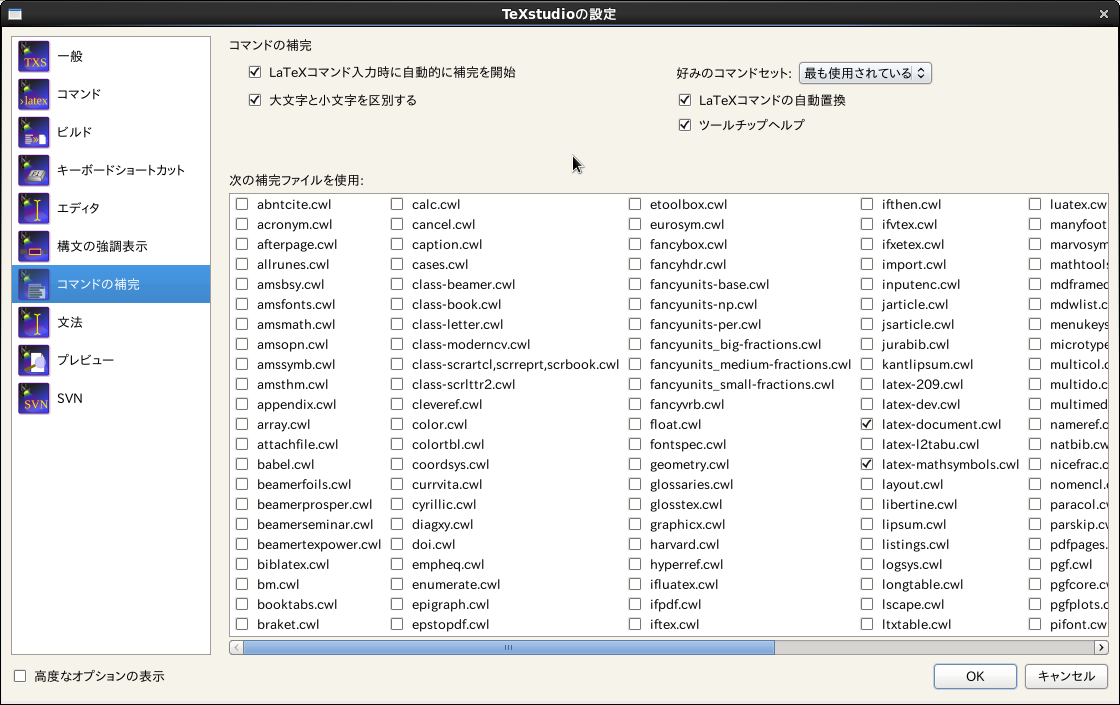
\includegraphics[width=.8\linewidth]{configure_completion.png}
  \caption{補完の設定}
\end{figure}

\section{ショートカットの設定}

ショートカットは、「現在のショートカット」または
「追加のショートカット」の場所でダブルクリックを行うことにより変更できる。
ショートカットは、ドロップダウンリストから選択するか、
直接テキストとして入力することができる。
ショートカットを規定値に設定もしくは完全に除去するのであれば、
リストの最上部にある「\textless{}default\textgreater{}」
または「\textless{}none\textgreater{}」を選択すればよい。

\begin{figure}[H]
  \centering
  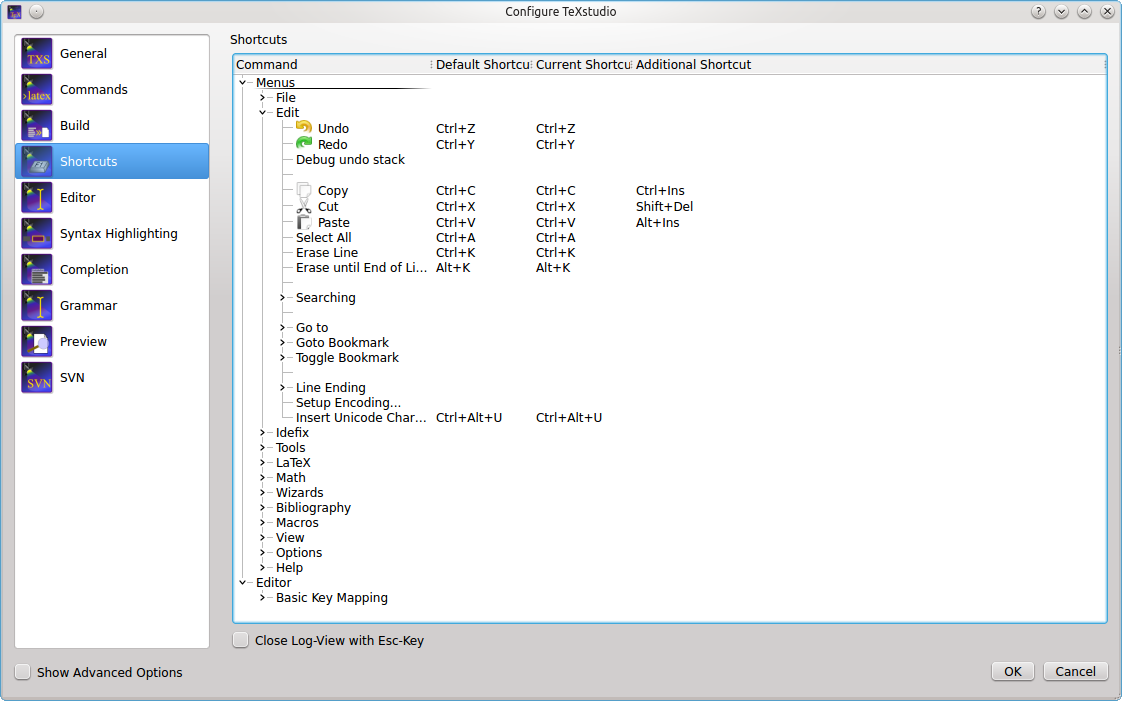
\includegraphics[width=.8\linewidth]{configure_shortcuts.png}
  \caption{ショートカットの設定}
\end{figure}

\section{Latex/Mathメニューの設定(高度なオプション)}

Math/Latexメニューはユーザーの好みに合わせることができる。
このメニューに対して、項目の名前を変更したり、
新規にLaTeXコードを追加したりすることが可能である。
各項目は、ダブルクリックすることで直接編集することができる。

\begin{figure}[H]
  \centering
  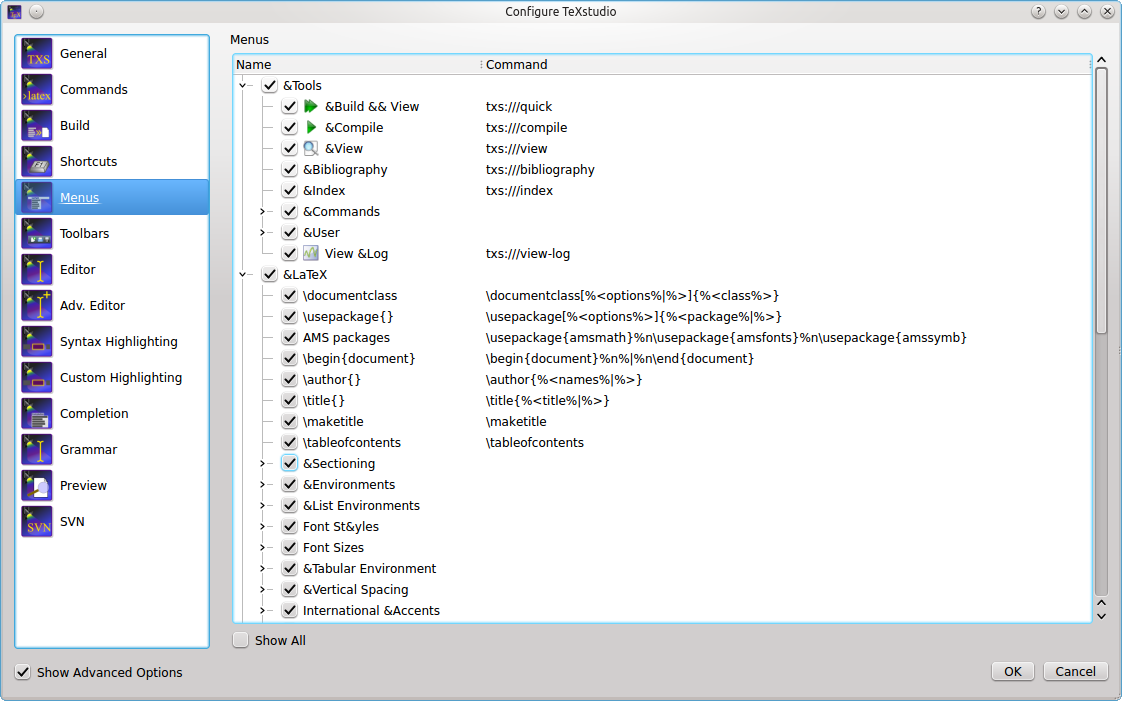
\includegraphics[width=.8\linewidth]{configure_customizeMenu.png}
  \caption{メニューのカスタマイズ}
\end{figure}

\section{カスタムツールバーの設定(高度なオプション)}

TXSにはカスタムツールバーがひとつ存在する。
このツールバーはLaTeX、Math、ユーザーメニューの要素から成り立っている。
これらの項目の多くにはアイコンがないので、
ユーザーが好きなアイコンを読み出すこともできる。
これは、設定ダイアログのカスタムツールバーリストで、
項目のコンテキストメニューから「別のアイコンの読み出し」をすることで可能となる。

\begin{figure}[H]
  \centering
  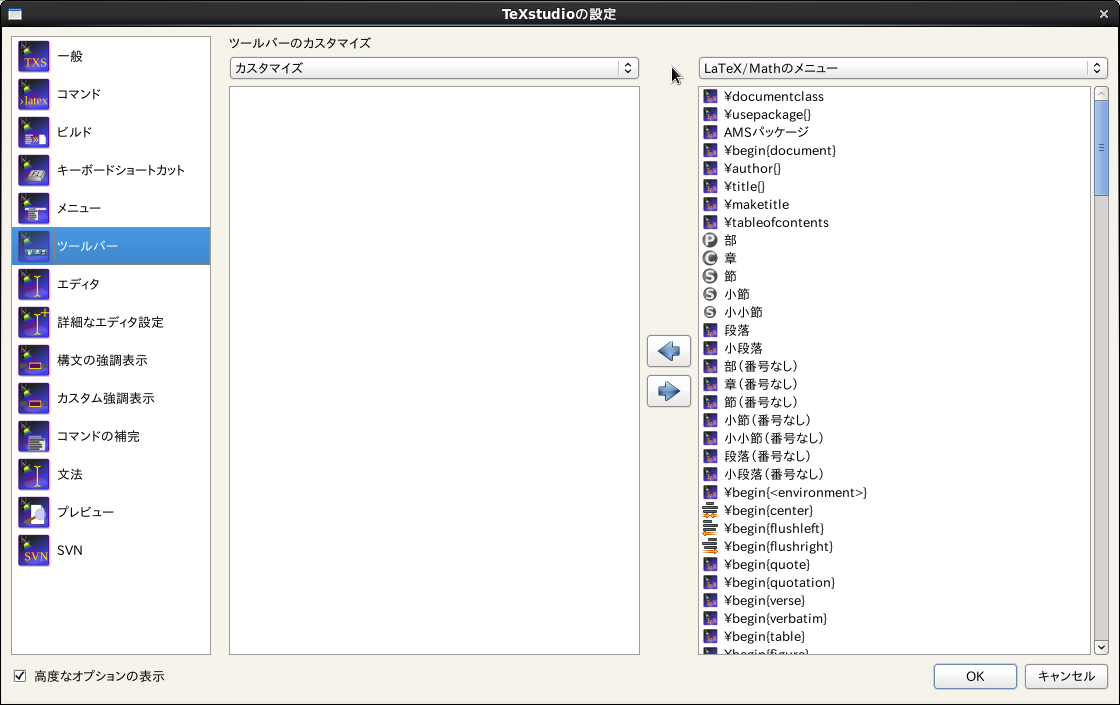
\includegraphics[width=.8\linewidth]{configure_customToolbar.png}
  \caption{ツールバーのカスタマイズ}
\end{figure}

\section{SVNサポートの設定}\label{sec:config_svn}

文章のバージョン管理を提供するため、TeXstudioではSVN(Subversion)を使用している。
これを利用するには、SVNコマンドラインツールがインストールされている必要がある。
LinuxとMac OSXでは通常SVNツールが(パッケージとして)すでに提供されており、
Windowsでは「SlikSVN」のインストールが推奨される。

下図のようなSVN設定ページの適切な欄に、
「svn」と「svnadmin」のコマンドへの完全なパスが設定されている必要がある。
更に、ユーザーはTeXstudioで提供される自動化の度合いを選択することができる。

「保存後に自動的にチェックインする」を選択すると、
TeXstudioが文書を保存するたびにSVNチェックインを行う。
従って文書作成の非常に完全な履歴が残ることとなる。
テキスト文書はディスクの空きスペースに比べて小さいので、
SVNのデータベースのサイズは問題にならない。
更に、ディレクトリがすでにSVNの制御下にある場合、
(「名前をつけて保存」で)新たに保存したファイルは自動的にSVNの制御下に追加される。
そうでない場合、
TeXstudioは現在のディレクトリ上での「SVNディレクトリの検索深度」の
ディレクトリ内でSVNの制御下のディレクトリを検索し、
サブディレクトリとTeX文書をSVNの制御下に追加する。
適切なディレクトリが見つからない場合、
リポジトリが「./repo」というディレクトリに自動的に作成され、文書が追加される。
従って、ユーザーはリポジトリ設定のための必要なコマンドを探す必要はない。
「自動チェックイン」を有効化した場合にのみこの機能は有効化される!

「最後の保存以前に戻すためにSVNリビジョンを用いる」を使うと、
TeXstudioはアンドゥを通常のように行うが、
内部記憶領域にアンドゥ可能なコマンドがそれ以上ない場合に、
文書をSVN履歴での一つ前のバージョンに変更する。
さらなるアンドゥコマンドでより古いリビジョンへ戻すことが可能である一方で、
「元に戻す」コマンドでより新しいバージョンへ変更できる。
これは直接メニューコマンドを通してSVNのリビジョンを選択することよりも
インタラクティブな手法である(
%\hyperref[SECTION33a]{4.4章}
\ref{sec:svnsupport}章\nameref{sec:svnsupport}参照)。

\begin{figure}[H]
  \centering
  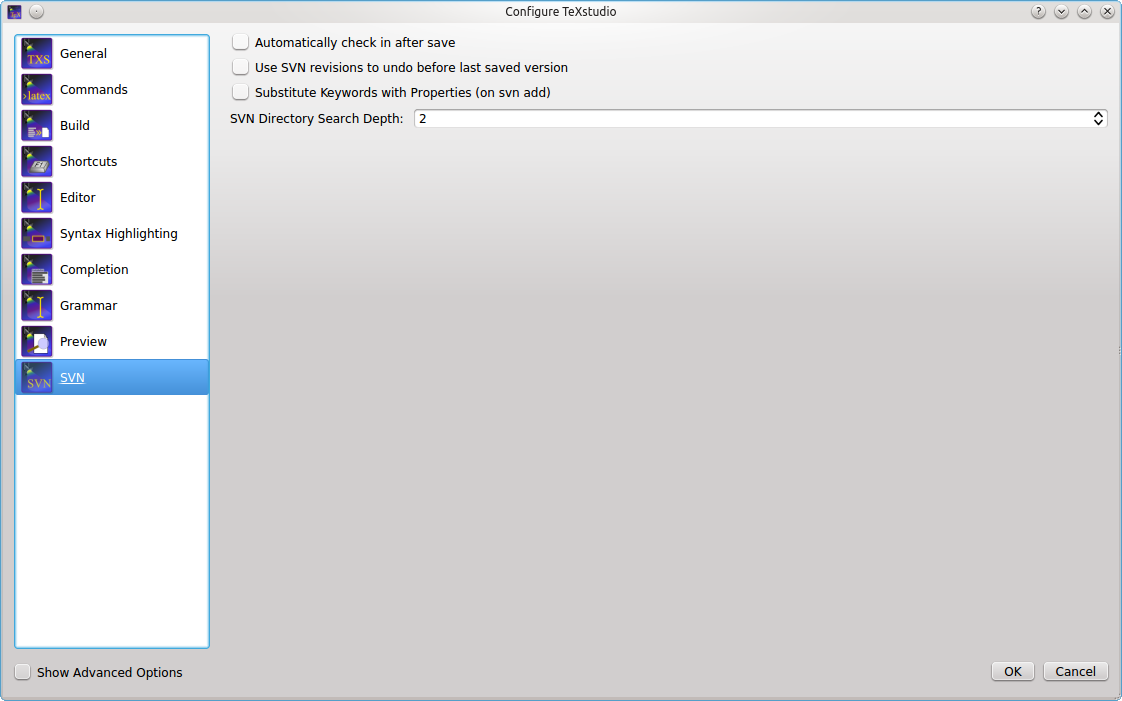
\includegraphics[width=.8\linewidth]{configure_svn.png}
  \caption{SVNの設定}
\end{figure}
